\chapter{Численное моделирование с пмощью кода COSY Infinity} \label{chpt:simulation}

\section{Фальш-сигнал} \label{sec:simulation-fake_signal}
Данная серия симуляций была проведена с целью подтвердить два тезиса
касательно систематической ошибки измерения частоты прецессии спина в
вертикальной плоскости, вызванной неточностью установки E+B элементов:
\begin{enumerate*}[1)]
	\item индуцированный МДМ-эффект зависит только от среднего значения
	угла наклона элементов, но не от  конкретной последовательности
	углов (т.е. отсутствует эффект \emph{геометрической фазы}); и
	\item эта зависимость носит линейный характер.
\end{enumerate*}

Наклон элемента вокруг оптической оси моделировался путём добавления
после элемента спин-кика вокруг радиальной оси соответствующей
величины (см. раздел~\ref{sec:error_field_implementation}). Это
гарантирует сохранение замкнутой орбиты при введении наклонов, что
физически обусловлено появлением компенсирующего электрического поля 
спин-ротатора при его наклоне.

Симуляция была проведена следующим образом: мы распределили наклоны
$\Theta_{tilt}$ E+B элементам FS структуры случайным образом. После
построения матриц перехода 3-го порядка, были вычислены разложения
Тейлора функций спин-тюна и оси прецессии спина (SPA). Члены нулевого
порядка этих разложений представляют собой спин-тюн и SPA референсной частицы.

Симуляция была проведена 11 раз; каждый раз углы наклона
спин-ротаторов выбирались из нормального распределения
$N(\mu_0\cdot(i-5), \sigma_0)$, где $\mu_0 = 10\cdot \sigma_0 =
10^{-4}$ рад, $i\in\lbrace0,\dots, 10\rbrace$. Результаты представлены
на Рисунке~\ref{fig:Linearity_test_shifting_gauss}.

\begin{figure}[!h]
	\centering\hfill
	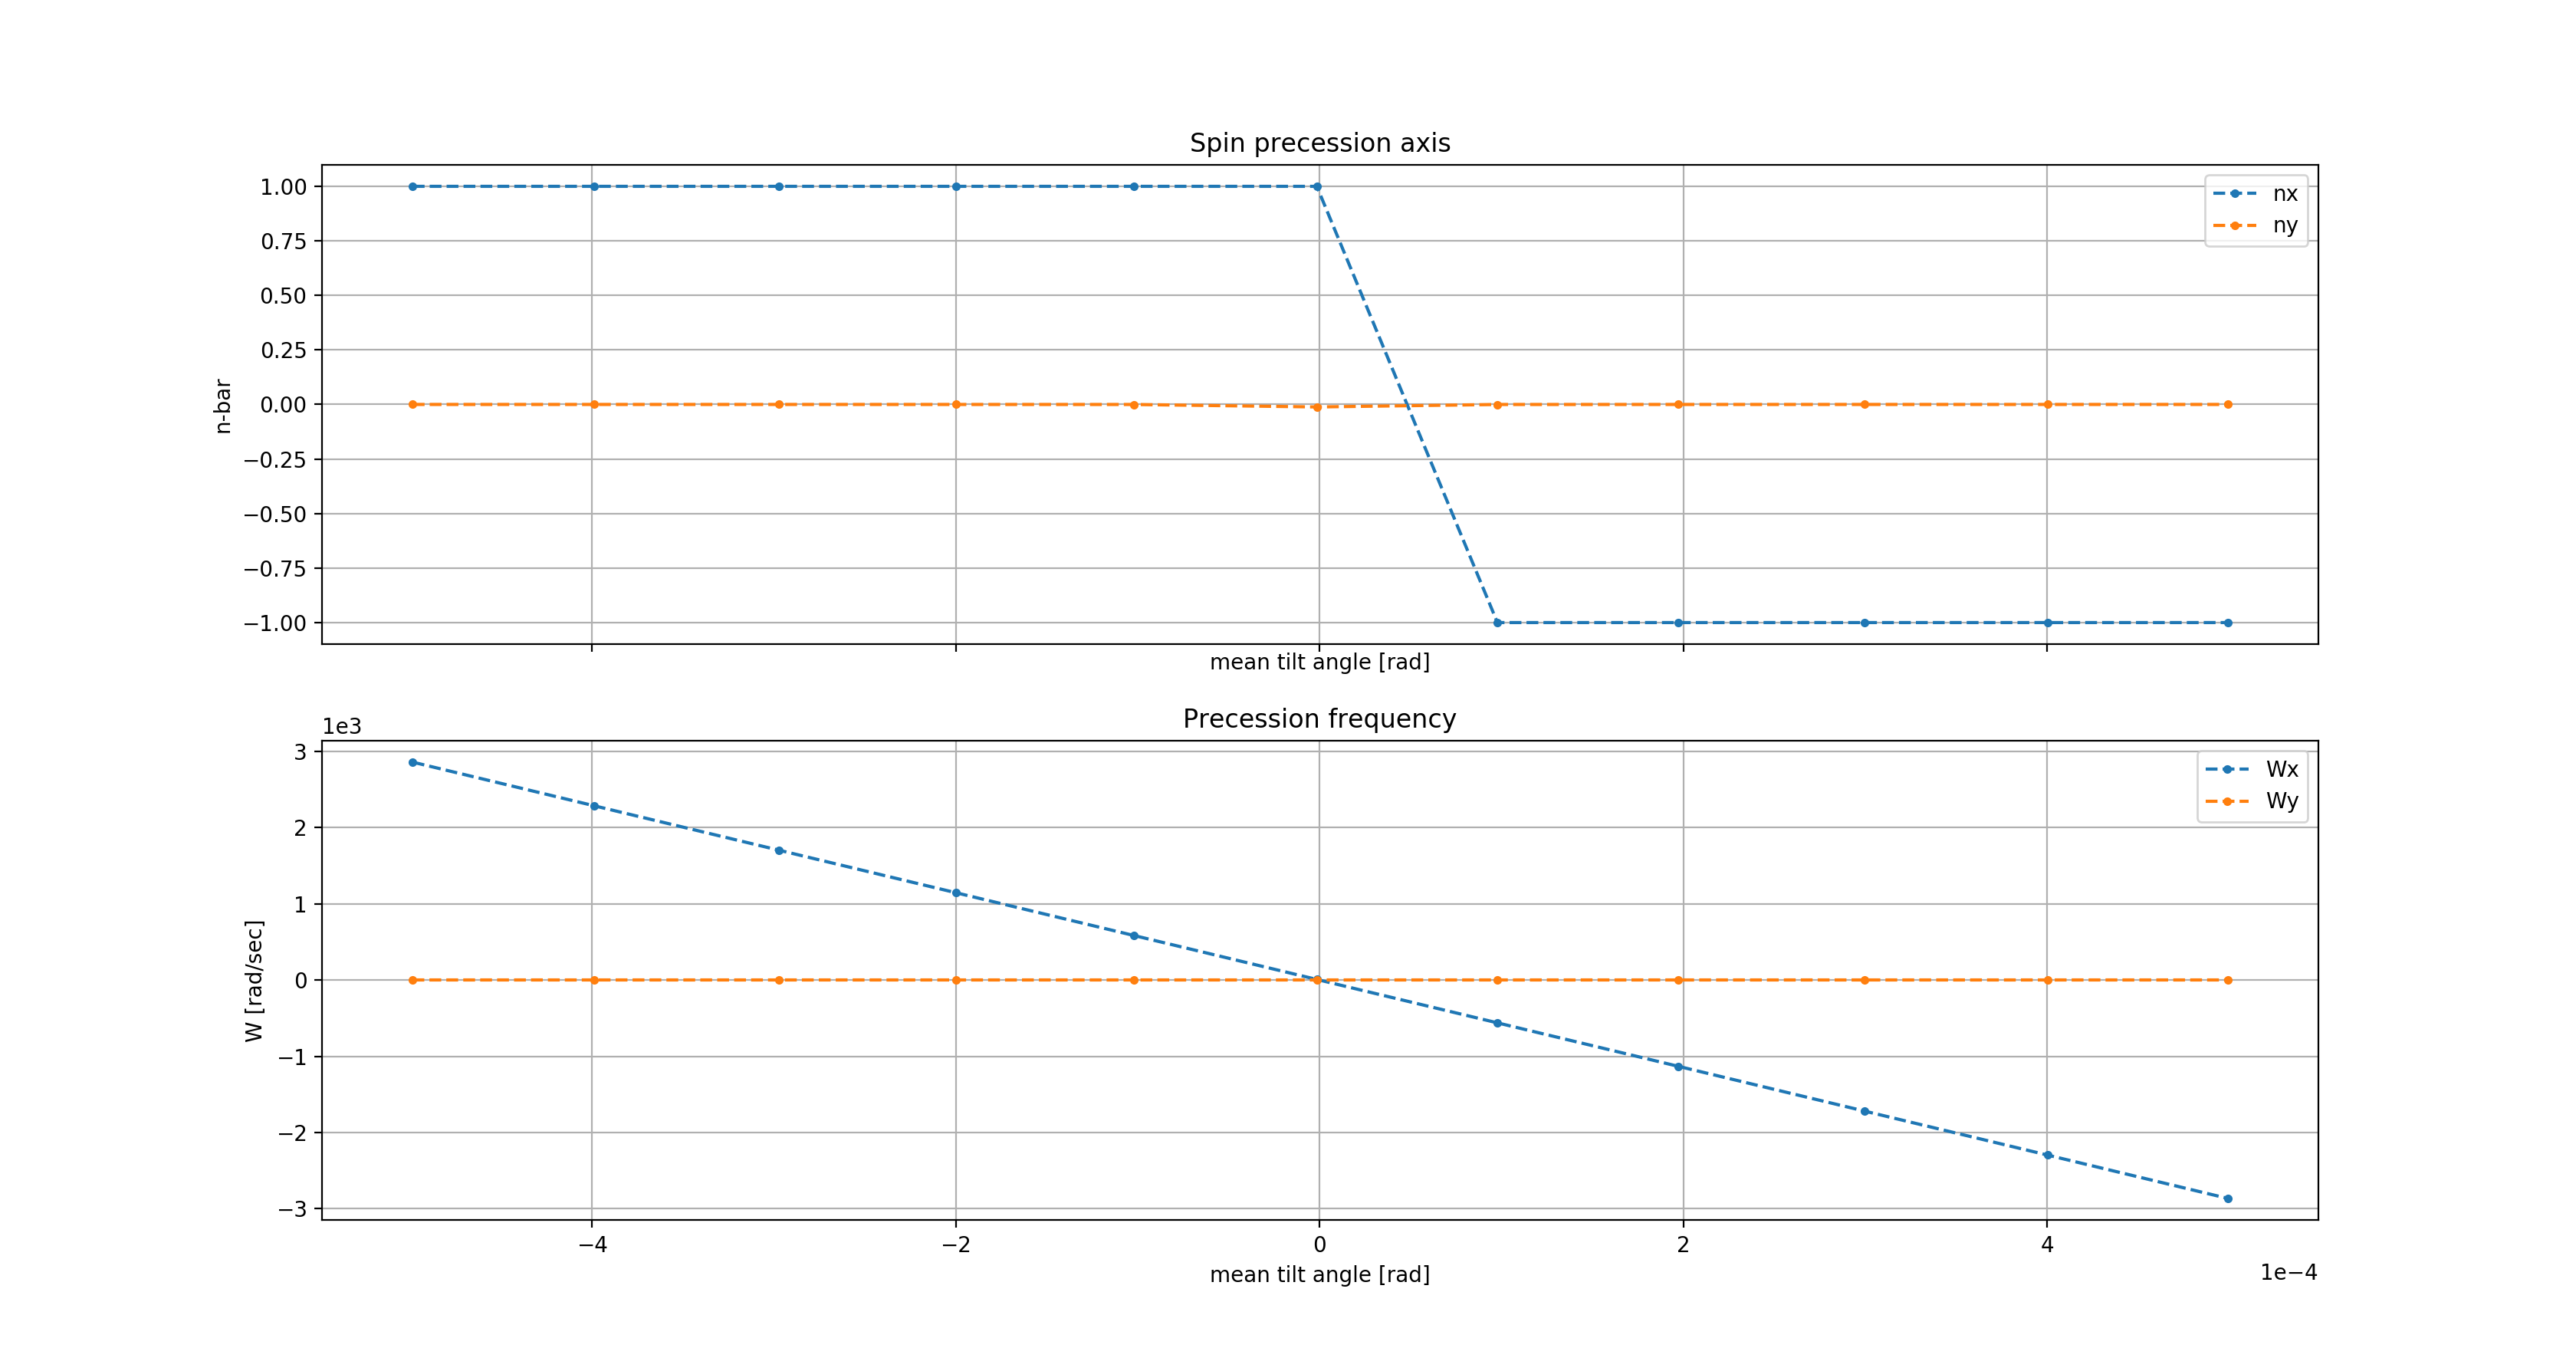
\includegraphics[width=\textwidth]{images/fake_signal_sim/linearity_test_shifting_gauss}
	\hfill
	\legend{Цветом различаются радиальная (синий) и вертикальная (оранжевый) компоненты векторов $\bar n$, $\vec\W$.}
	\caption{Компоненты $\bar n_x$, $\bar n_y$ оси прецессии спина, и частоты прецессии $\W_x$, $\W_y$ для неидеальной FS структуры, а зависимости от среднего угла наклона E+B элементов.\label{fig:Linearity_test_shifting_gauss}}
\end{figure}

На Рисунке~\ref{fig:Linearity_test_compensated} изображены результаты теста, в котором E+B элементы попарно повёрнуты на противоположные углы (три случайные пары), а один элемент повёрнут на угол
$\mu_i = (i-5)\cdot 10^{-6}$ рад, $i\in\lbrace0,\dots,10\rbrace$. Обе симуляции были выполнены на энергии
270.0092 МэВ.\footnote{На этой энергии ось прецесии спина и спин-тюн
	не определены в системе координат связанной с пучком, использованной
	COSY INFINITY, для идеальной структуры. Это соответствует ситуации
	когда спин не прецессирует ни в какой плоскости (горизонтальной или
	вертикальной), что есть условие замороженного спина в идеальной структуре.}

\begin{figure}[!h]
	\centering\hfill
	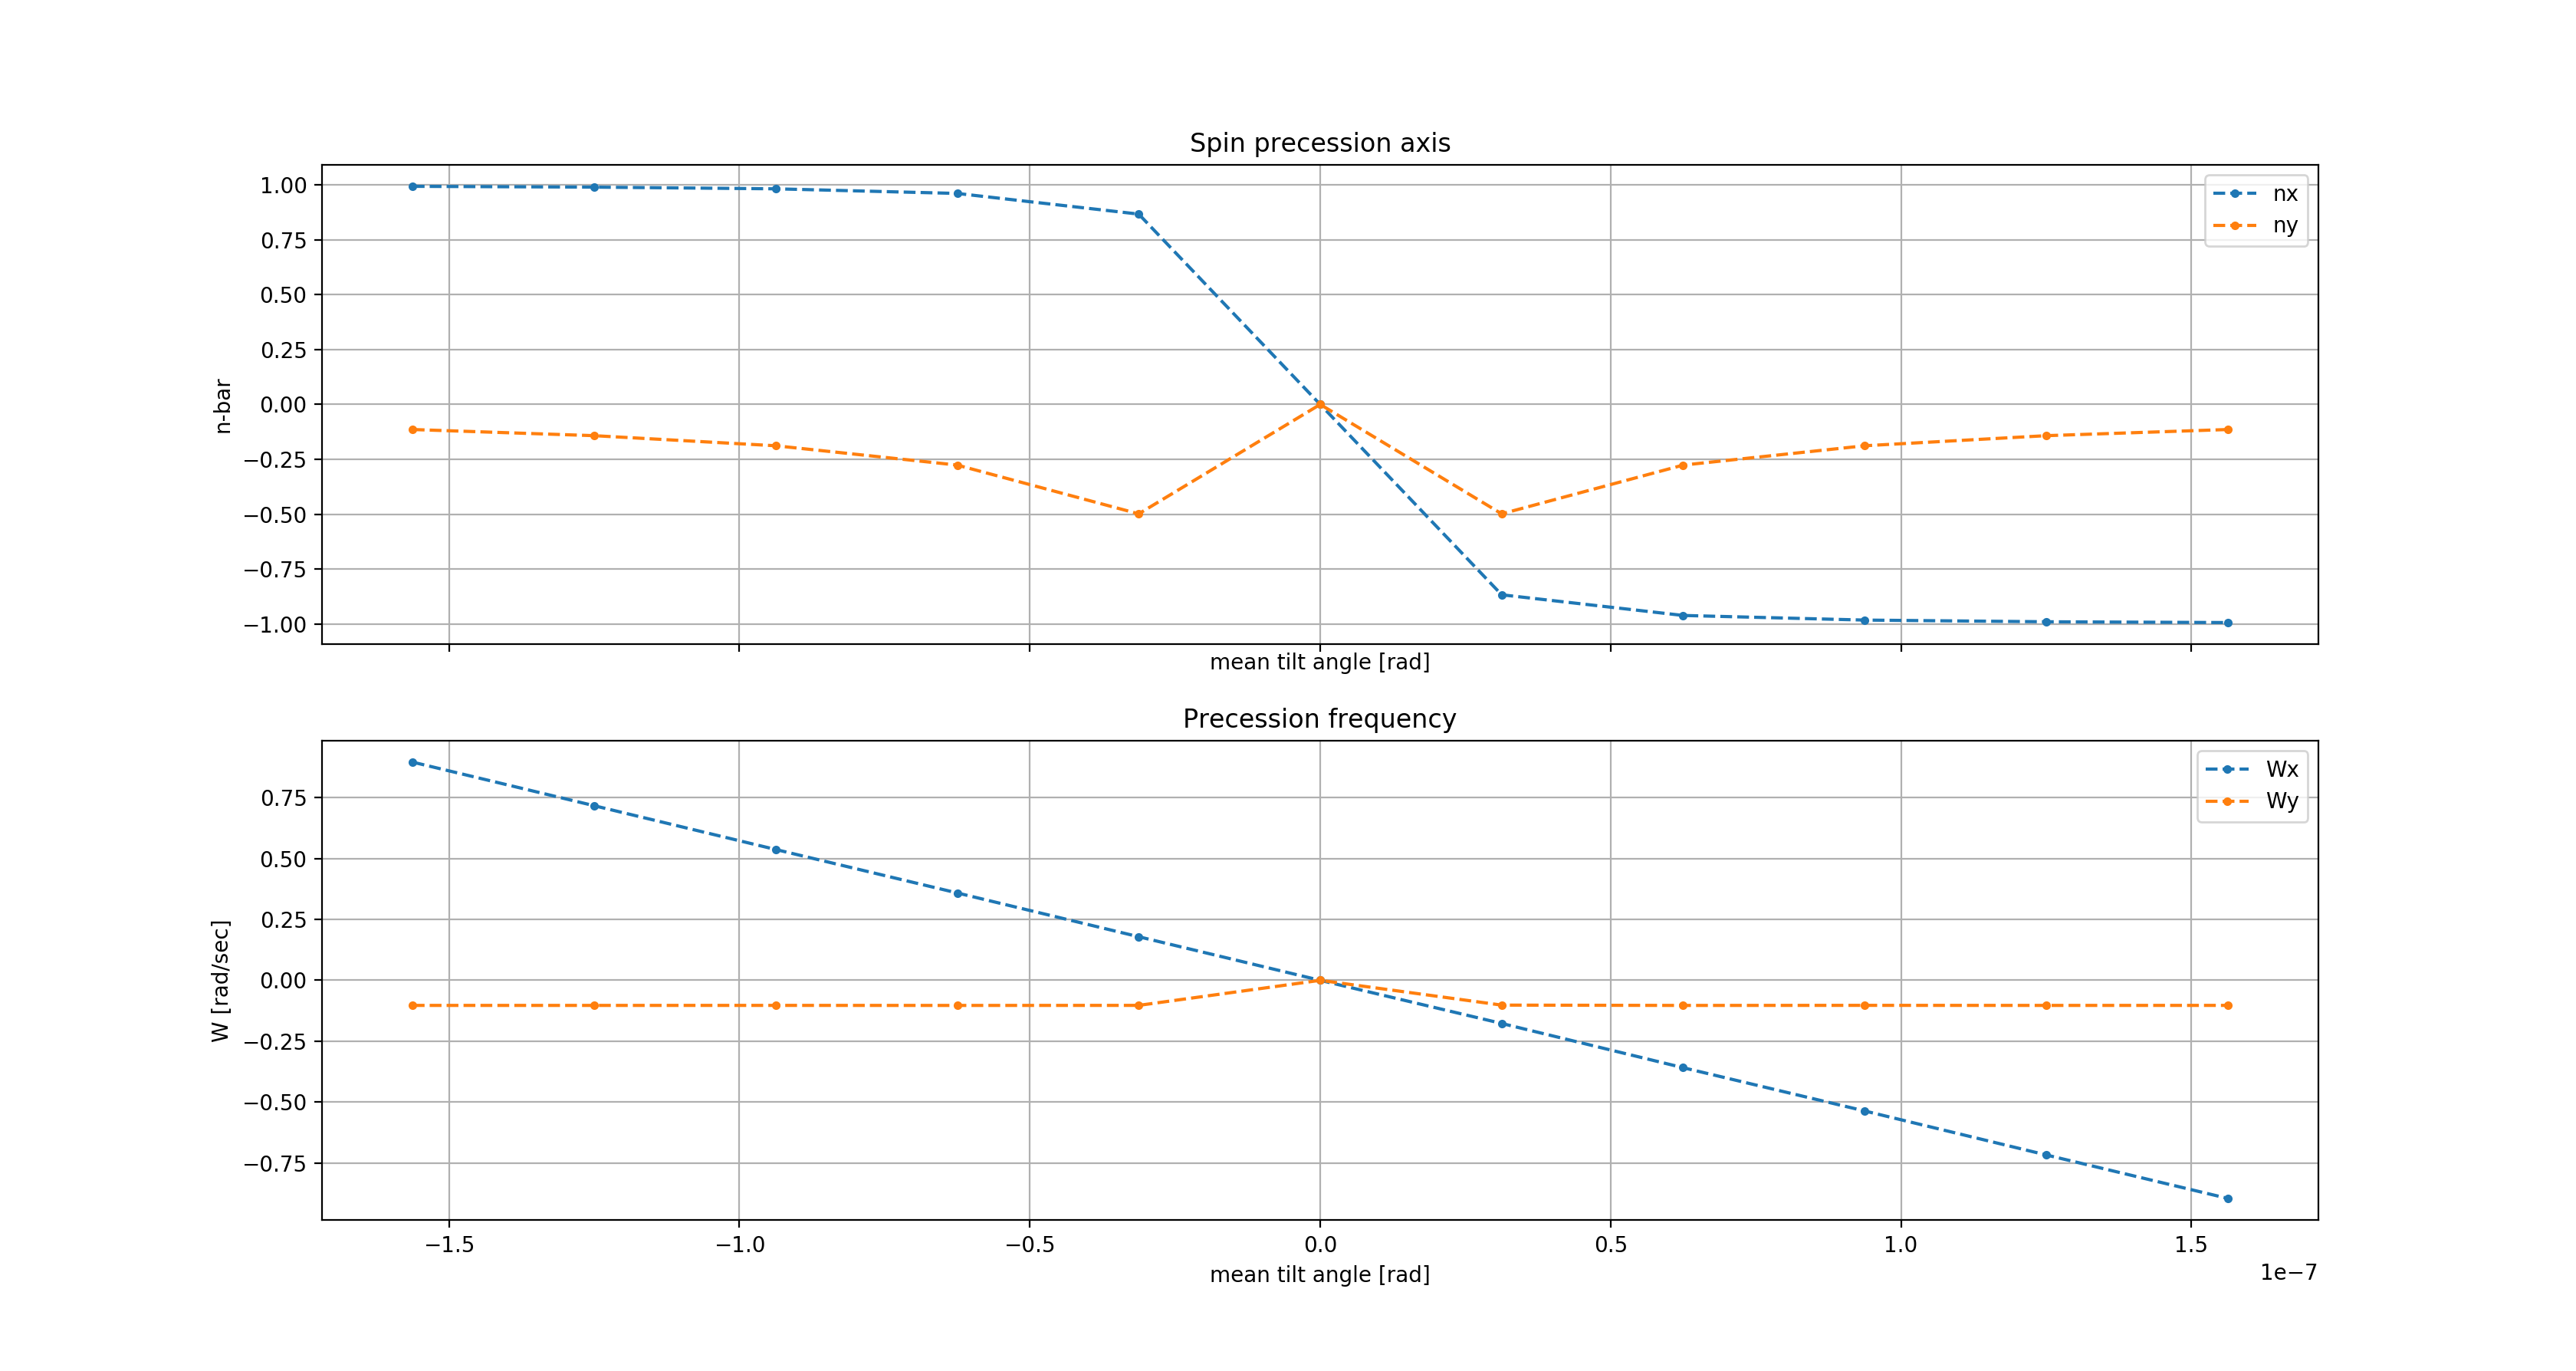
\includegraphics[width=\textwidth]{images/fake_signal_sim/linearity_test_compensated+microrad}
	\hfill
	\legend{Цветом различаются радиальная (синий) и вертикальная (оранжевый) компоненты векторов $\bar n$, $\vec\W$.}
	\caption{Компоненты оси прецессии спина и частоты прецессии в зависимости от среднего угла наклона спин-ротаторов.\label{fig:Linearity_test_compensated}}
\end{figure}

\section{Декогеренция и её оптимизация}\label{sec:decoherence_simulations}
При проведении нижеследующих тестов симулировалась инжекция
плоского, гауссовского пучка в структуру с замороженным
спином. Инжектируемые пучки состояли из 30 частиц, распределённых в
плоскости $y-z$ как $y\sim N(y_0, 0.1)$ [мм]; $x,d =
0$. Оффсет $y_0$ варьировался в диапазоне $[-1, +1]$ мм. Начальное
направление спин-векторов всех частиц --- продольное: $\vec S(t=0) = (0,0,1)$.

Также в структуре варьировалось значение градиента GSY секступоля,
модулирующего декогеренцию в вертикальной плоскости. GSY менялся в
диапазоне $[GSY0 - 5\cdot10^{-3}, GSY0 + 5\cdot10^{-3}]$, где
$GSY0=-2.5\cdot 10^{-3}$ --- оптимальное значение градиента для идеальной структуры.

На каждое значение градиента приходится 10 инжекций.

Пучок инжектировался на энергии 270.0092 МэВ (строгий FS), в структуру
с неточно-установленными E+B спин-ротаторами. 

Наклоны E+B элементов
генерировались из распределения $N(0, 5\cdot10^{-4})$ радиан. При
симуляциях использовалась энергия строгой заморозки спина, а не,
например, близкая к ней 270 МэВ, для того, чтобы минимизировать
вертикальную компоненту оси прецессии. Матрицы перехода орбитального и спинового движений строятся до  третьего
порядка разложения ряда Тейлора, чтобы обеспечить устойчивость
процедуры TSS COSY Infinity.~\cite{COSYINF:BeamPhysMan}

Далее ансамбль начальных значений, представляющий пучок, трекается
через структуру на протяжении $1.2\cdot10^6$ оборотов, что
примерно эквивалентно 1.2 секундам. Каждые 800 оборотов производится
запись необходимых для анализа данных.

Собираемые данные: 
\begin{enumerate*}[\itshape a\upshape)]
	\item результаты вычислений процедуры TSS: спин-тюн $\nu_s$ и компоненты вектора оси инвариантного спина $\bar n$, а также
	\item компоненты спина $(S_X, S_Y, S_Z)$, и фазового пространства $(X,A,Y,B,T,D)$.
\end{enumerate*}

Из данных по компонентам спина вычисляется поляризация банча по
формуле
\begin{equation}\label{eq:polarization_formula}
\vec P = \frac{\sum_i\vec s_i}{|\sum_i\vec s_i|}.
\end{equation}

Поляризация фиритуется функцией $f(t; a,f,\phi) = a\cdot \sin(2\pi\cdot
f\cdot t + \phi)$, оцениваются все три параметра $(\hat a, \hat f,
\hat\phi)$. 

\subsection{Симуляция эффекта подавления декогеренции спина в вертикальной плоскости при помощи секступолей}
На Рисунке~\ref{fig:ny_vs_y0_GSY} представлена зависимость вертикальной компоненты оси прецессии частицы от её смещения от референсной орбиты в вертикальном направлении. Из Рисунка~\ref{fig:ny_vs_y0_GSY_full} видно, что существует некоторое значение градиента секступоля, при котором $\bar n_y(y) = \bar n_y(0)$ для всех частиц в диапазоне $\pm 1$ мм от референсной орбиты. Обратим внимание на то, что на Рисунке~\ref{fig:ny_vs_y0_GSY_zoom} наблюдается чётность функции $\Delta\bar n_y \equiv \bar n_y(y) - \bar n_y(0)$.

\begin{figure}[h!]
	\centering
	\hfill
	\subbottom[Полный диапазон.\label{fig:ny_vs_y0_GSY_full}]{%
		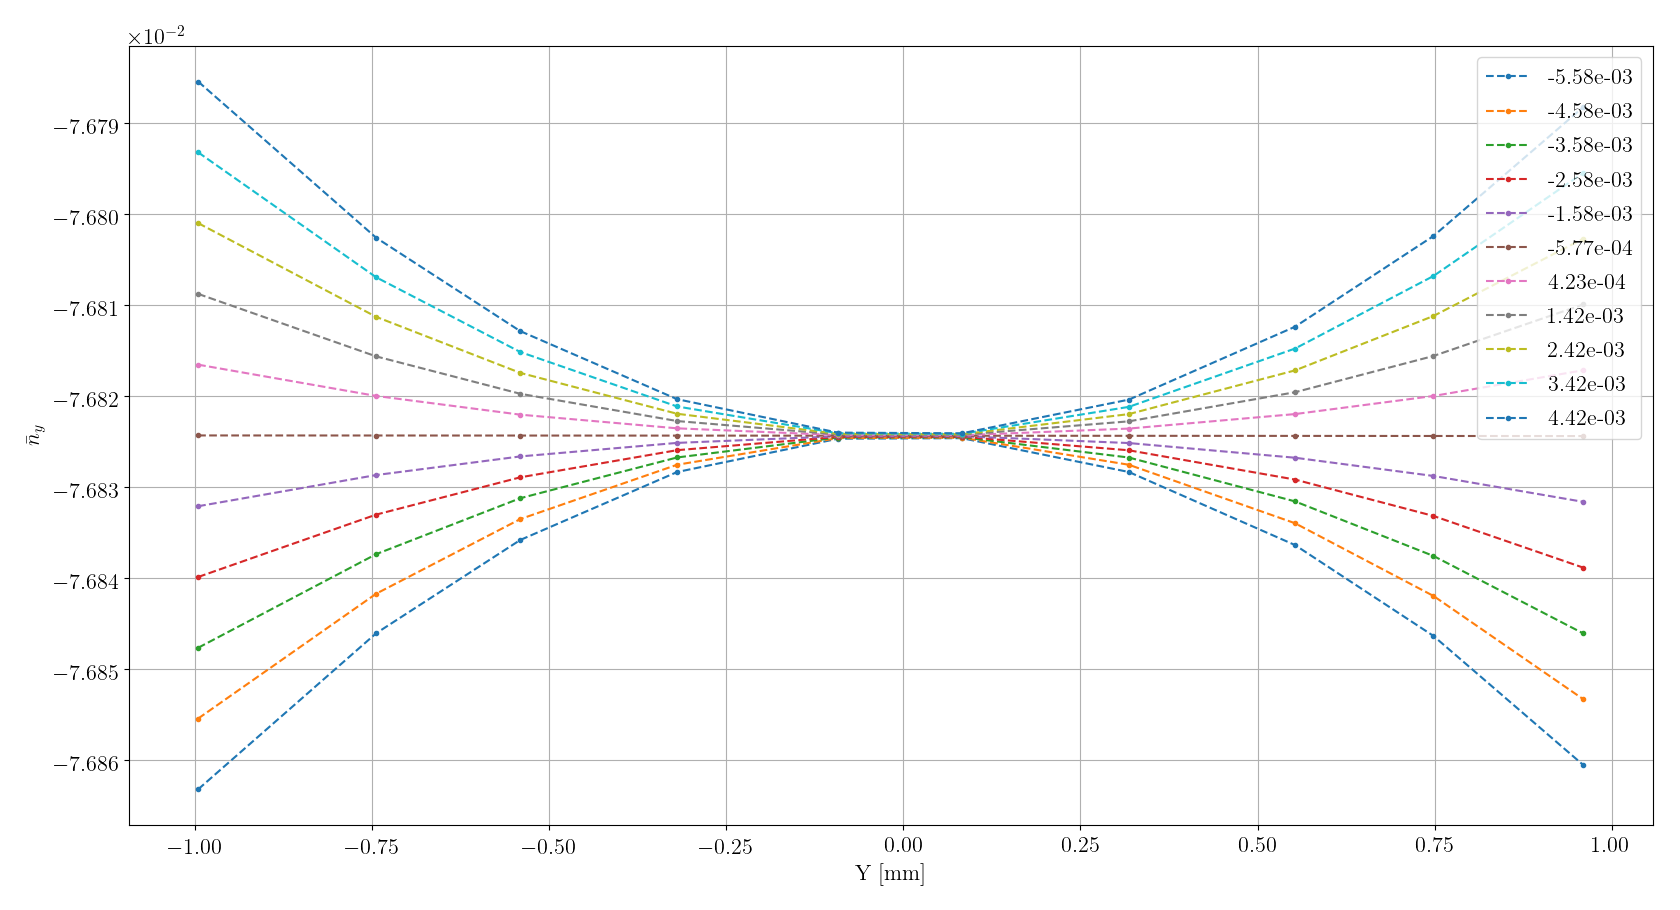
\includegraphics[width=\linewidth]{images/decoh_sim/ny_vs_offset}}
	\hfill
	\subbottom[Деталировка кривой при оптимальном значении GSY.\label{fig:ny_vs_y0_GSY_zoom}]{%
		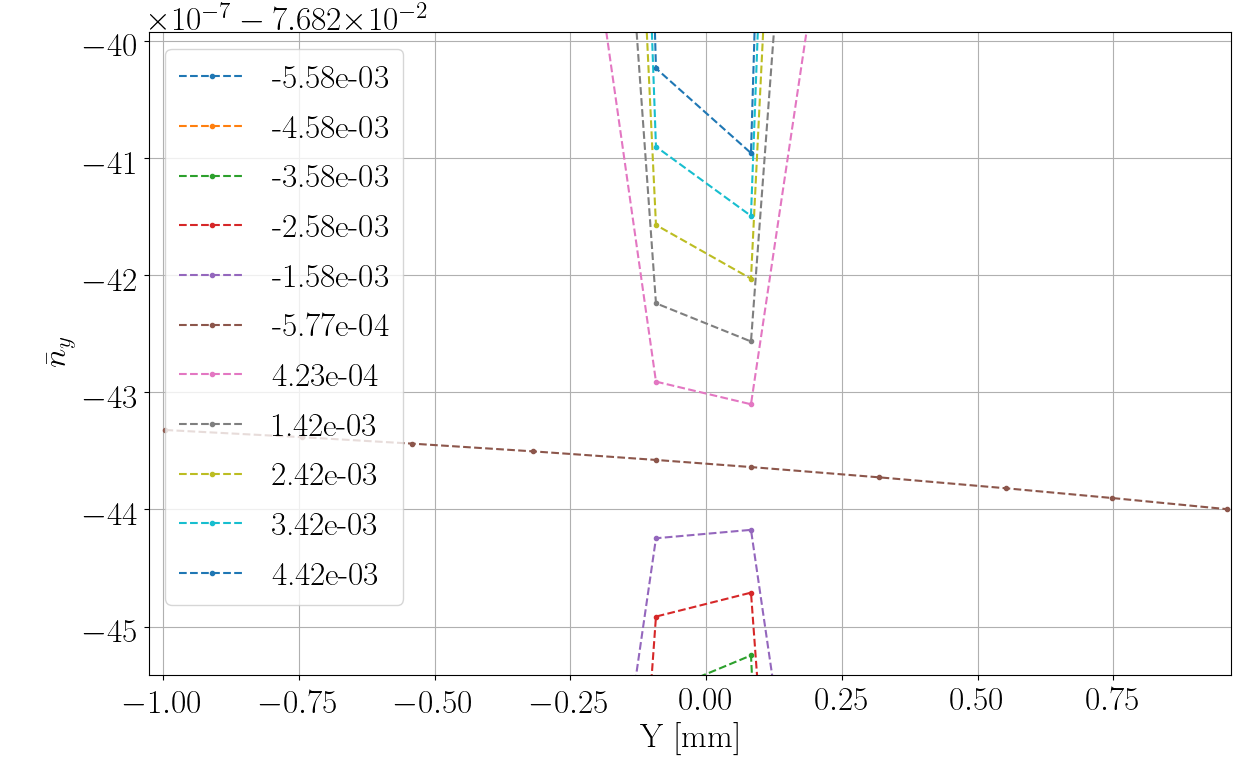
\includegraphics[width=\linewidth]{images/decoh_sim/ny_vs_offset_zoom}}
	\hfill
	\legend{Цветом обозначены данные для различных значений градиента GSY Y-секступоля.}
	\caption{Вертикальная компонента $\bar n_y$ оси прецессии спина в зависимости от смещения частицы от референсной орбиты.\label{fig:ny_vs_y0_GSY}}
\end{figure}

На Рисунке~\ref{fig:spin_tune_vs_y0_GSY} представлена зависимость спин-тюна от вертикального смещения частицы от референсной орбиты. Видно, что $\Delta\nu_s \equiv \nu_s(y) - \nu_s(0)$ --- нечётная функция.
\begin{figure}[h!]
	\centering
	\hfill
	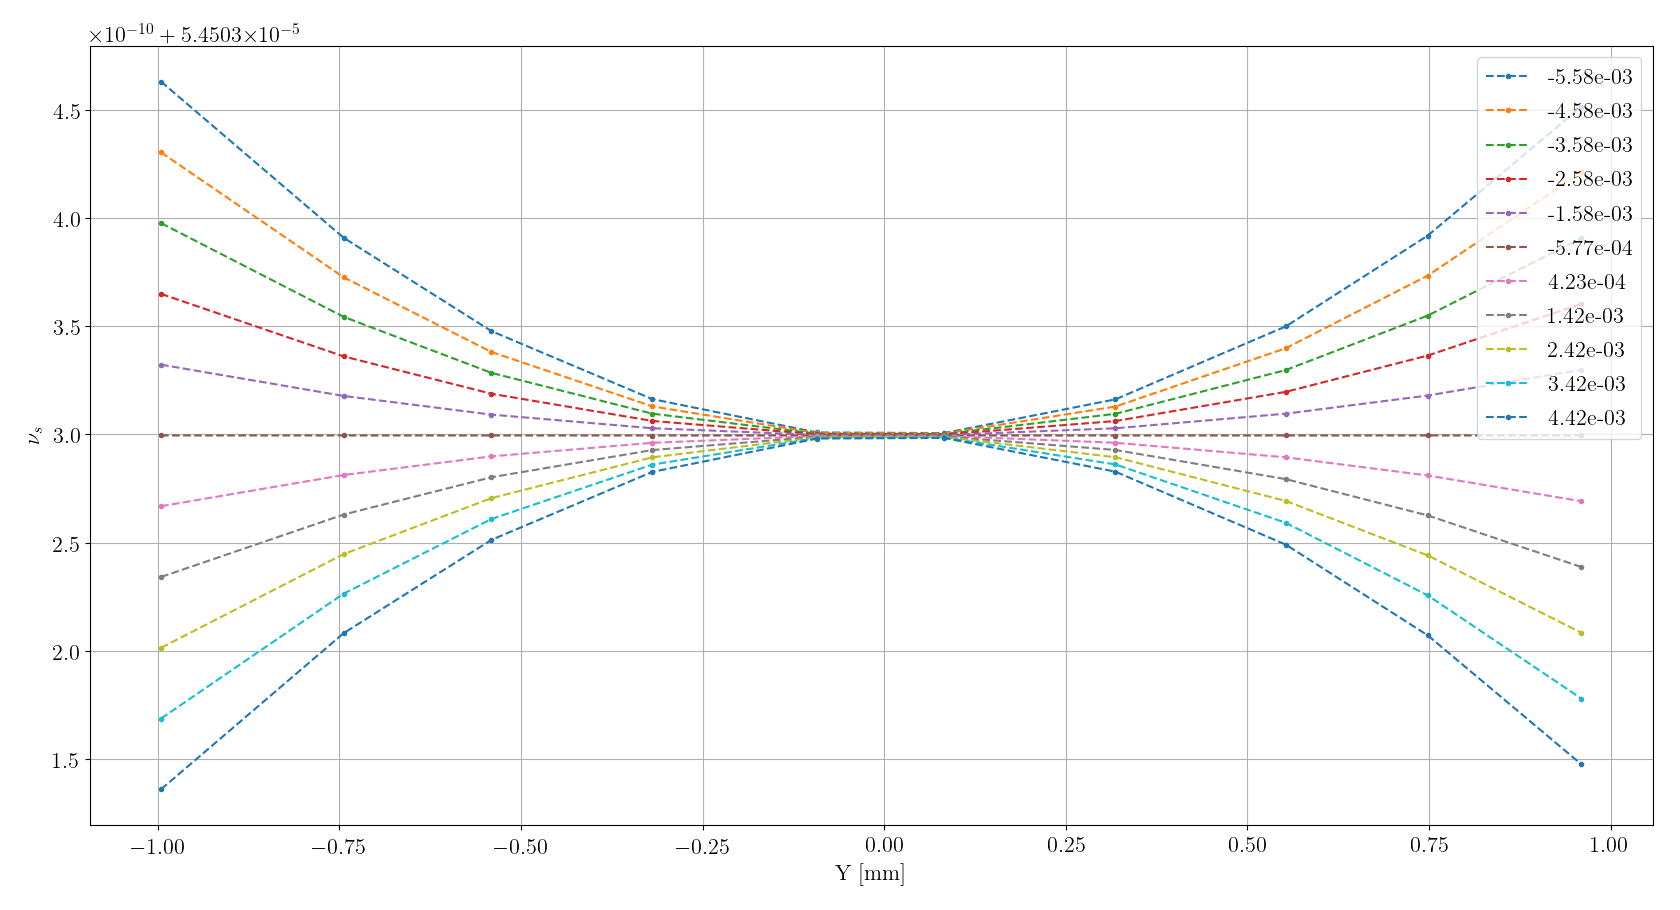
\includegraphics[width=\linewidth]{images/decoh_sim/spin_tune_vs_offset}
	\hfill
	\legend{Цветом обозначены данные для различных значений градиента GSY Y-секступоля.}
	\caption{Спин-тюн $\nu_s$ в зависимости от смещения частицы от референсной орбиты.\label{fig:spin_tune_vs_y0_GSY}}
\end{figure}

На Рисунке~\ref{fig:freq_y_vs_y0} представлена зависимость оценки частоты колебаний вертикальной компоненты поляризации банча, вычисленной по формуле~\eqref{eq:polarization_formula}, в зависимости от его начального смещения, для трёх значений градиента GSY. Из Рисунка~\ref{fig:freq_y_vs_y0_zoom} видно, что функция $\Delta\hat f \equiv \hat f(y) - \hat f(0)$--- нечётная, как и $\Delta\nu_s$.
\begin{figure}[!h]
	\centering
	\hfill
	\subbottom[Полный диапазон.\label{fig:freq_y_vs_y0_full}]{%
		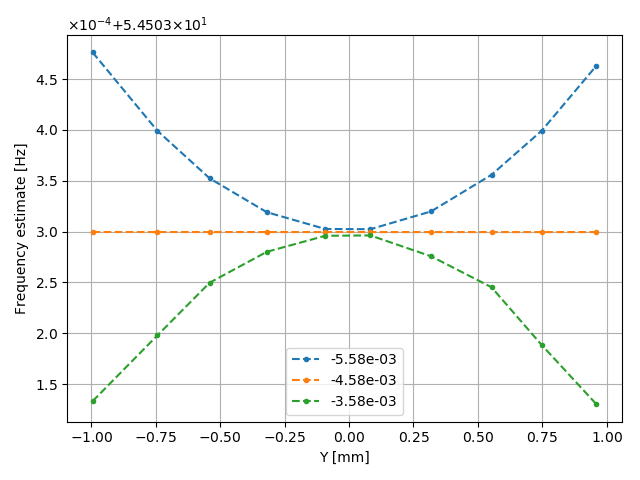
\includegraphics[width=\linewidth]{images/decoh_sim/FreqY_vs_offset}}
		\hfill
	\subbottom[Деталировка кривой при оптимальном значении градиента GSY Y-секступоля.\label{fig:freq_y_vs_y0_zoom}]{%
			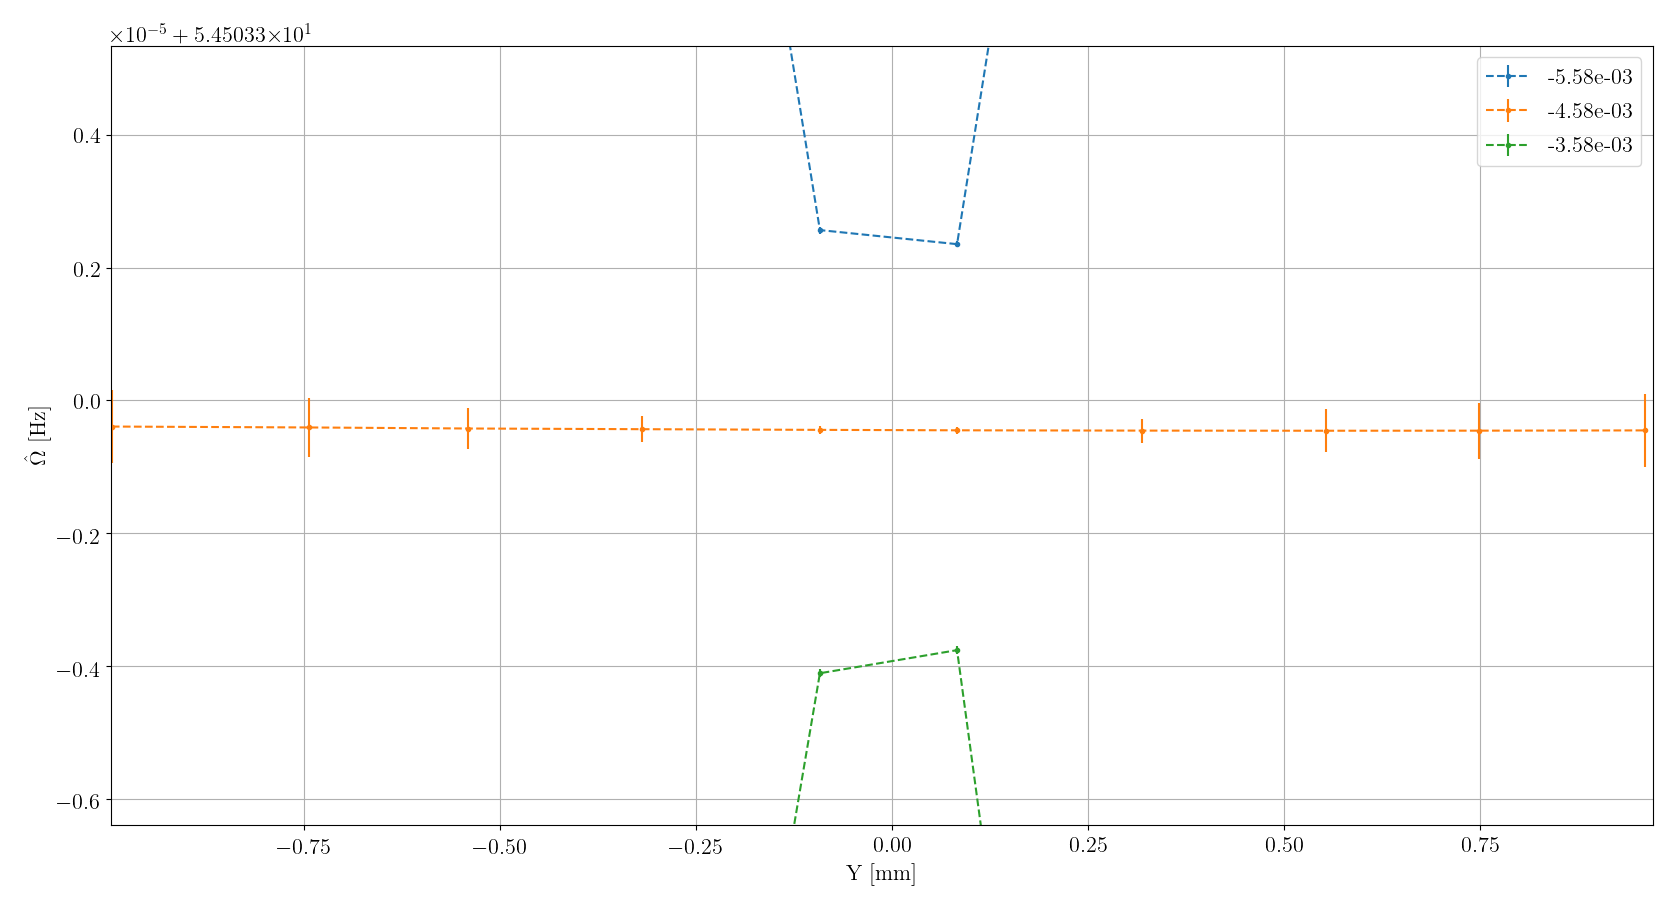
\includegraphics[width=\linewidth]{images/decoh_sim/FreqY_vs_offset_zoom}}
		\hfill
	\legend{Цветом обозначены кривые при различных значениях градиента GSY Y-секступоля.}
	\caption{Оценка частоты колебаний вертикальной компоненты поляризации в зависимости от начального смещения пучка от референсной орбиты.\label{fig:freq_y_vs_y0}}
\end{figure}

\subsection{Исследование зависимости оценки частоты прецессии поляризации банча от спин тюна и прецессии оси стабильного спина}\label{sec:SpinTune_and_SPA_dependence}

На Рисунке~\ref{fig:ny_vs_turn} представлена вертикальная компонента $\bar n$ для частиц с оффсетами,
соответственно.: [1.02749, 1.02937, 1.02840] мм. Мы наблюдаем быстрые осцилляции вокруг некоторого среднего уровня. Этот средний уровень имеет параболическую зависимость от вертикального смещения частицы (см. Рисунок~\ref{fig:mean_tune_axis}). Быстрые осцилляции вызваны бетатронным движением (см. Рисунок~\ref{fig:ny_on_traj}).

\begin{figure}[h!]
	\centering
	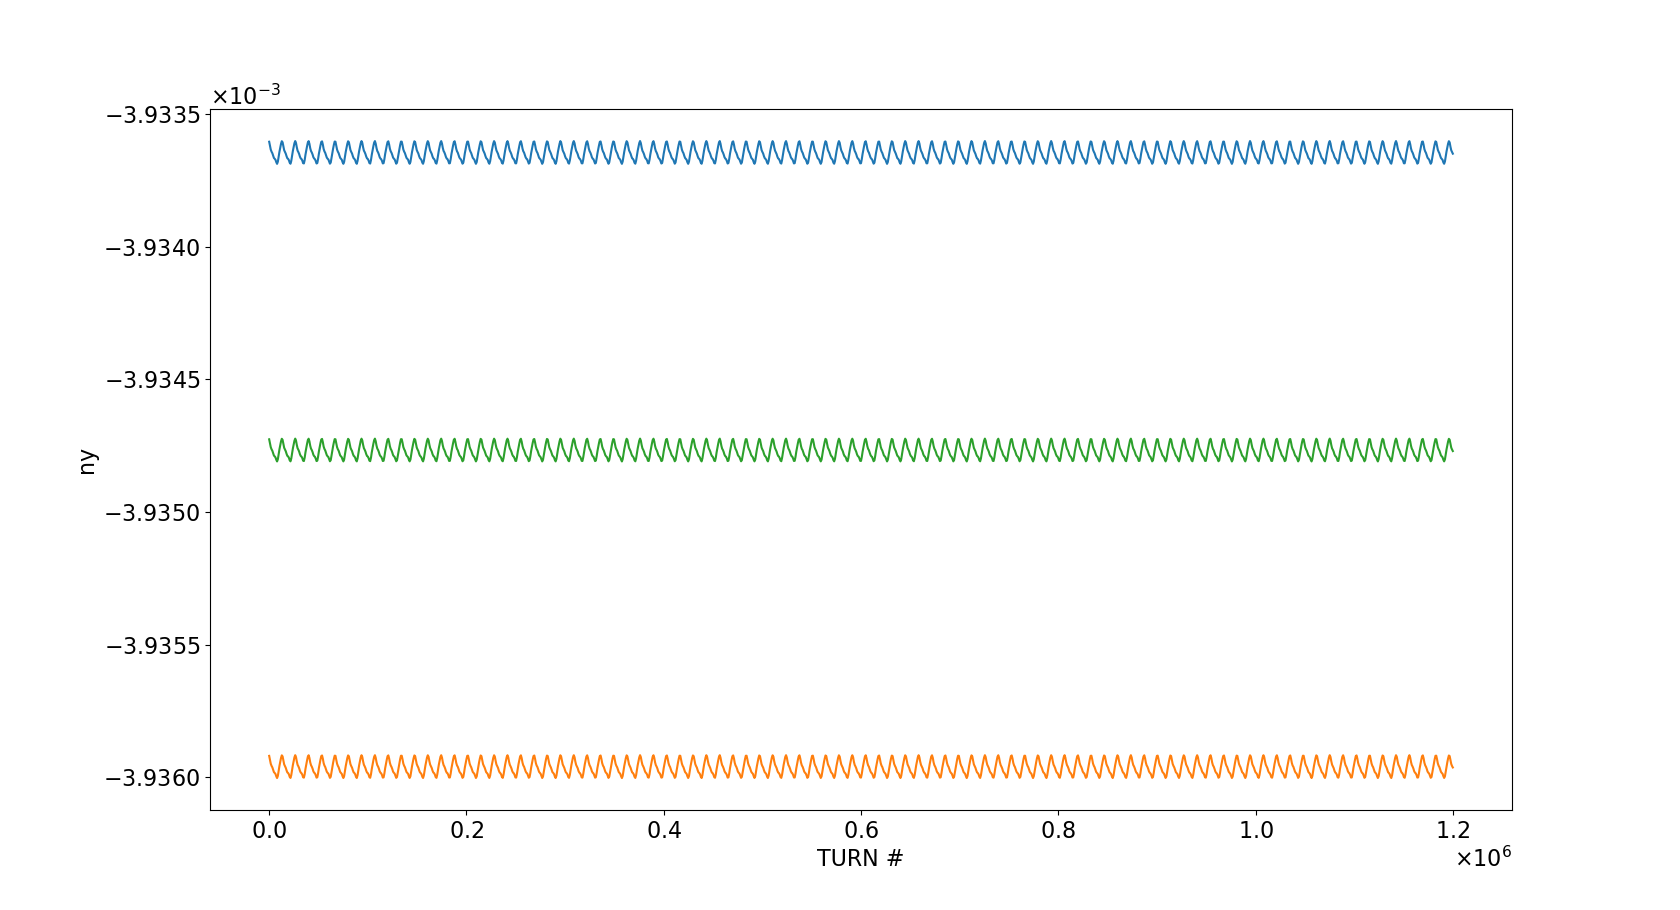
\includegraphics[width=\linewidth]{images/decoh_sim/ny_vs_turn}
	\caption{Зависимость $\bar n_y$ от номера оборота частицы в ускорителе.\label{fig:ny_vs_turn}}
\end{figure}

На Рисунке~\ref{fig:mean_tune_axis} показана зависимость средних уровней компонент оси прецессии спина и спин-тюна друг от друга. Видно, что величина спин-тюна и направление оси прецессии спина жёстко связаны между собой. В связи с этим следует вывод, что использование секступольных полей выравнивает не только скорости вращения спинов частиц вокруг их собственных осей прецессии в некотором диапазоне вокруг замкнутой орбиты, но также и направления самих осей. 
\begin{figure}[h!]
	\centering\hfill
	\subbottom[Средний уровень спин тюна в зависимости от вертикального сдвига пучка]{
		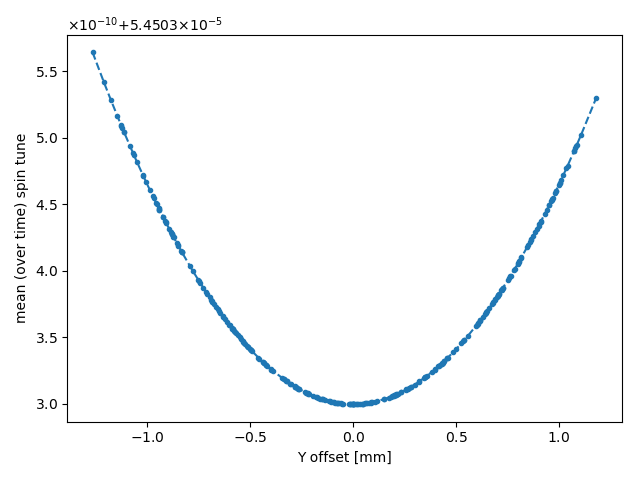
\includegraphics[width=\linewidth]{images/decoh_sim/mean_spin_tune_vs_y_offset}}
	\hfill
	\subbottom[Связь средних уровней компонент $\bar n$ и спин тюна]{%
		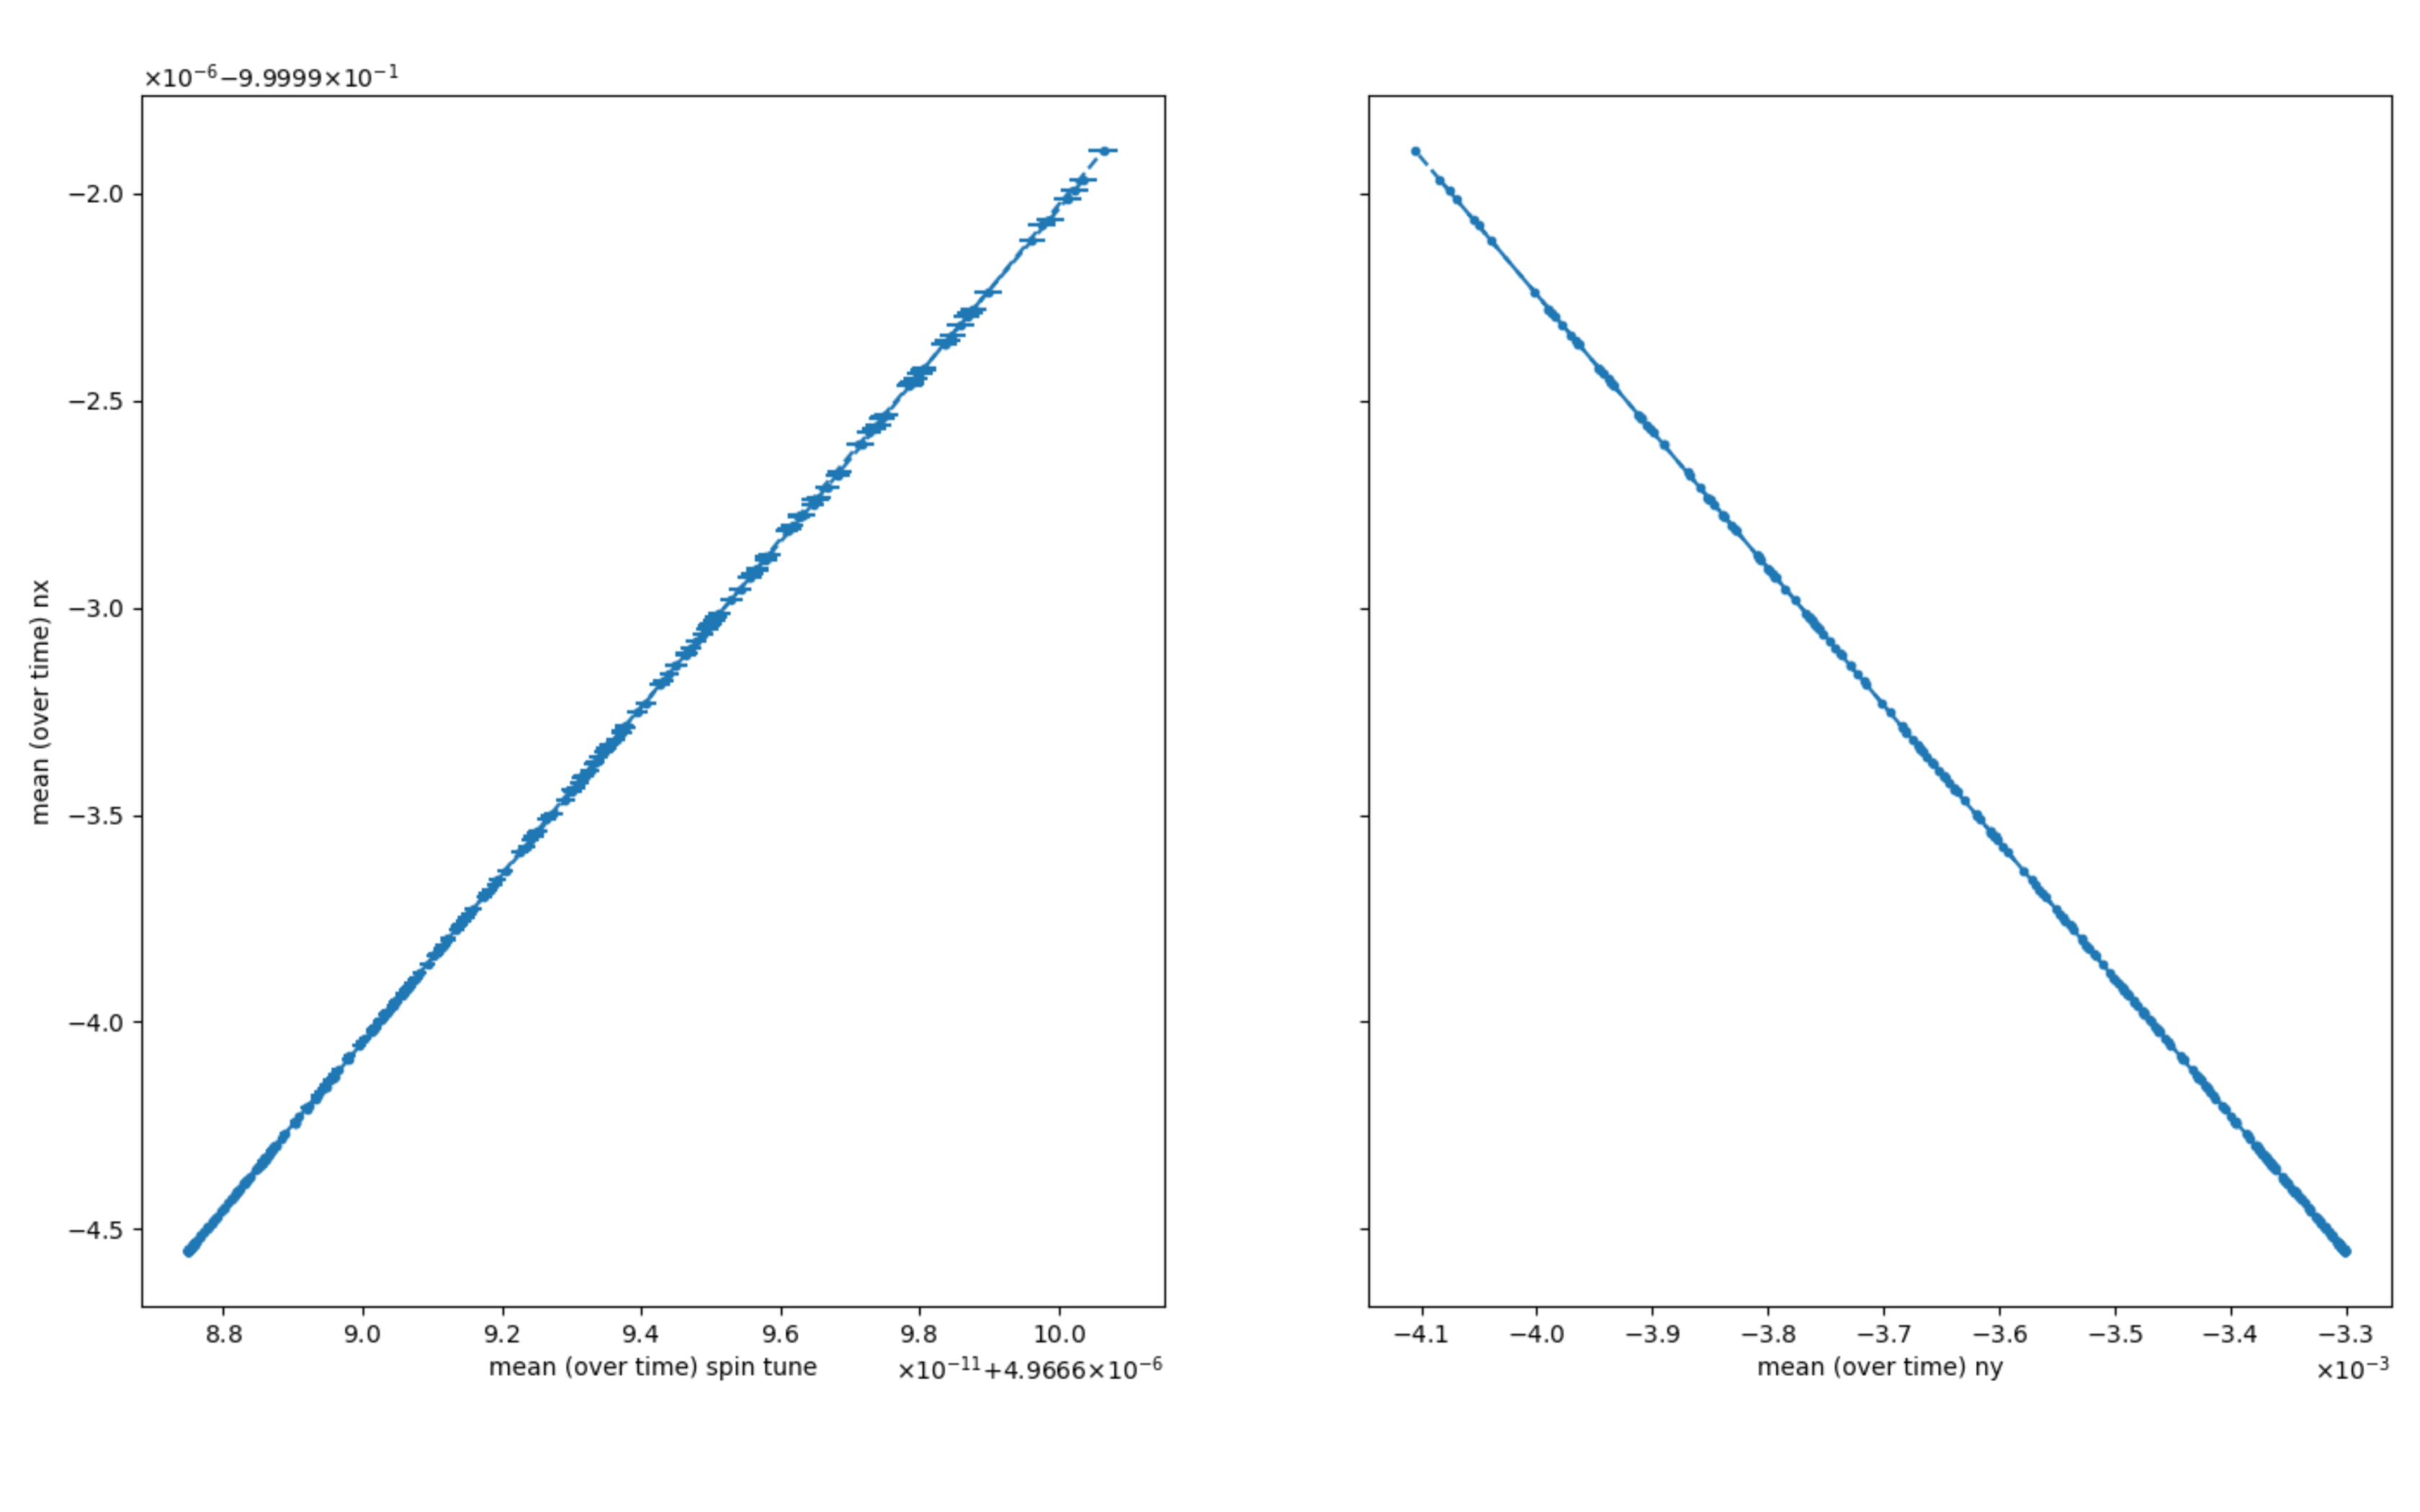
\includegraphics[width=\linewidth]{images/decoh_sim/mean_n_bar_vs_spin_tune}}
	\hfill
	\caption{Средние уровни спин тюна и оси стабильного спина в зависимости от начального вертикального сдвига пучка и друг друга.\label{fig:mean_tune_axis}}
\end{figure}

На Рисунках~\ref{fig:spin_tune_on_traj} и~\ref{fig:ny_on_traj} изображены, соответственно, спин-тюн и вертикальная компонента оси прецессии спина, вычисленные на траекториях частиц в неидеальном ускорителе, в случае с выключенными и включенными секступолями, подавляющими декогеренцию в вертикальной плоскости. 
\begin{figure}[!h]
	\centering
	\subbottom[С выключенными секступолями.]{%
	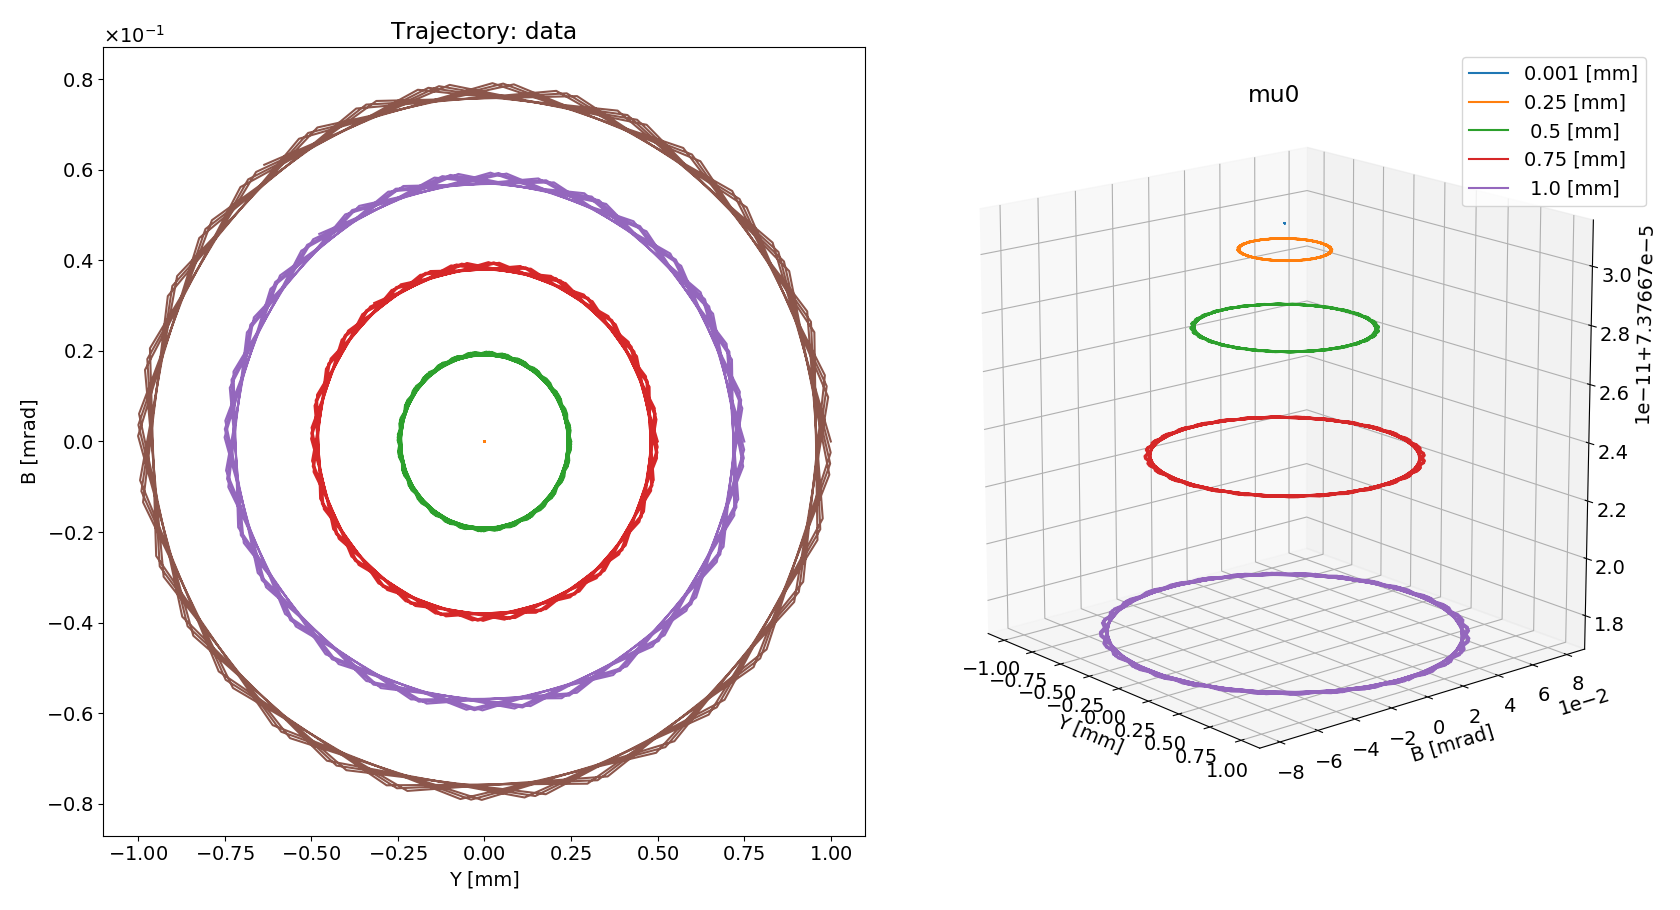
\includegraphics[width=\linewidth]{images/decoh_sim/SPIN_TUNE_VS_YB_DATA_TRAJ_UNOPTIM}}
	\hfill
	\subbottom[С включенными секступолями.]{%
	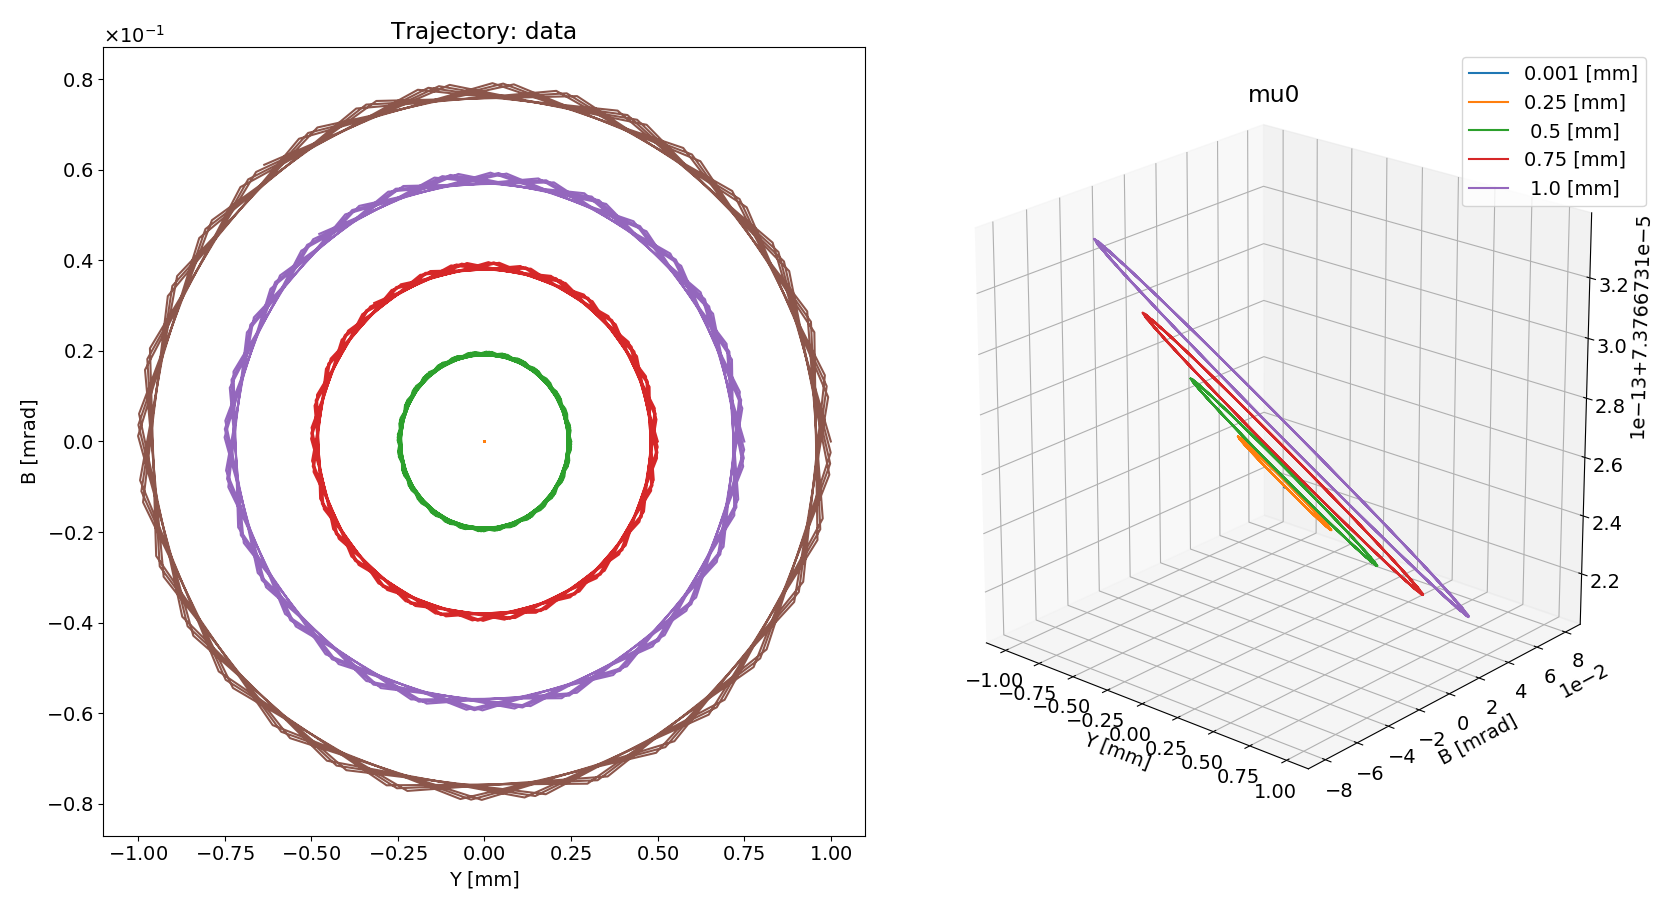
\includegraphics[width=\linewidth]{images/decoh_sim/SPIN_TUNE_VS_YB_DATA_TRAJ_OPTIM}}
	\hfill
	\caption{Траектории и спин-тюны частиц в неидеальной FS-труктуре.\label{fig:spin_tune_on_traj}}
\end{figure}

\begin{figure}[!h]
	\centering
	\subbottom[С выключенными секступолями.]{%
		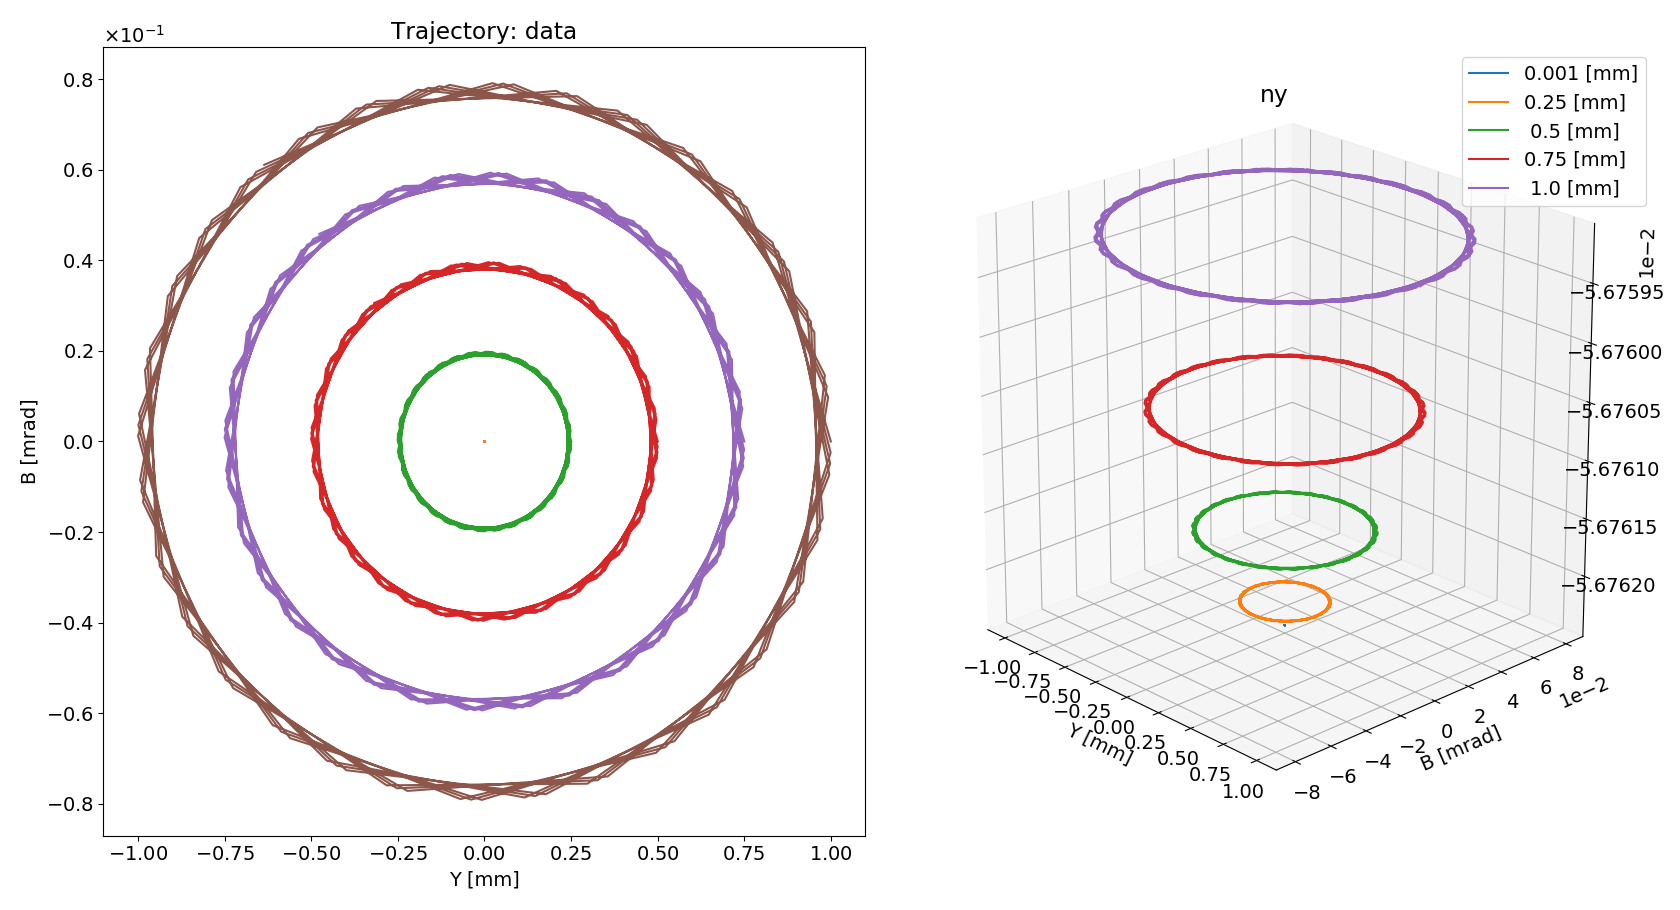
\includegraphics[width=\linewidth]{images/decoh_sim/NY_VS_YB_DATA_TRAJ_UNOPTIM}}
	\hfill
	\subbottom[С включенными секступолями.]{%
		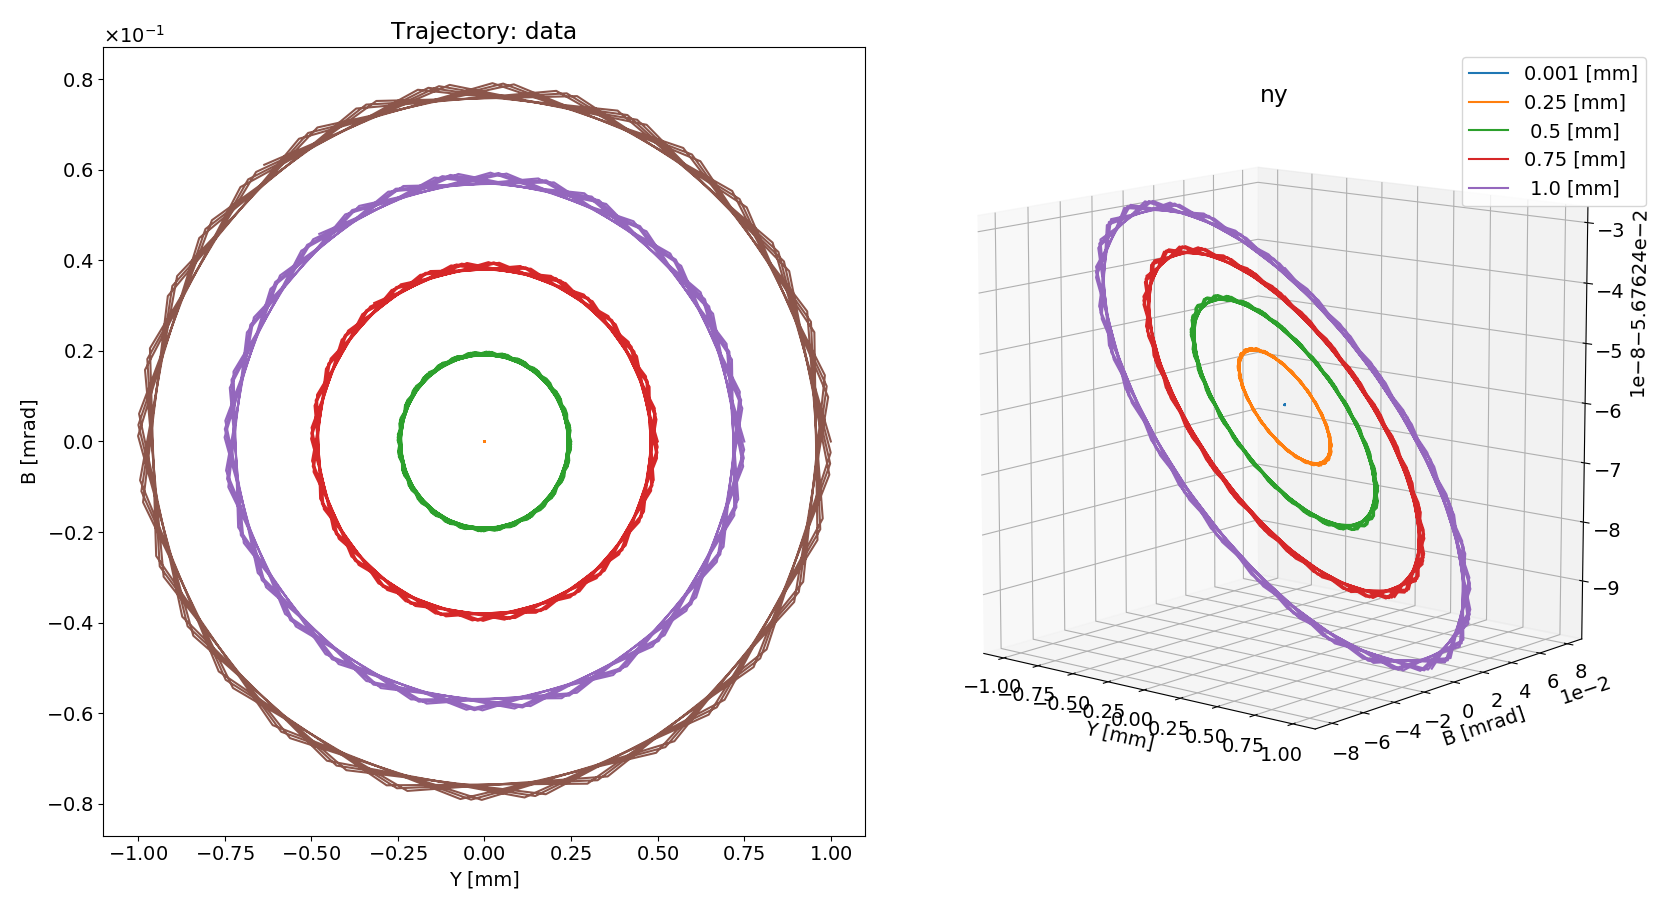
\includegraphics[width=\linewidth]{images/decoh_sim/NY_VS_YB_DATA_TRAJ_OPTIM}}
	\hfill
	\caption{Траектории и вертикальная компонента оси прецессии частиц в неидеальной FS-труктуре.\label{fig:ny_on_traj}}
\end{figure}

\section{Смена полярности ведущего поля} \label{sect3_2}

\clearpage
